
\subsubsection{24.10.14}

\begin{enumerate}
	\item The time of beginning and ending of the congregation:
	16:00 - 20:00
	\item Purposes of the congregation:
	\begin{enumerate}
	  \item Correct the problem with servo that rotates gripper for balls.
	  
	  \item Make by the aluminium sheet the slopes for ball and install to their at the robot.
	  
    \end{enumerate}
    
	\item Work, that has been done:
	\begin{enumerate}
	  \item Problem with servo was corrected. The cause of it's appearance is the rotation of the servo with low speed which not enough to overcome of elastic force of couplers. It happened due to wrong value of power servo in the programme (value in which servo stops - 127 instead 135 that was in our programme).
      
      \item Aluminium sheet was sawn to strips of needed sizes.
      
      \item Slopes were installed to robot and tested. The result is positive.
      
      \item During the test of slopes was seen that when they faces with a rigid obstacle they bend. To prevent this were installed stops that made of the aluminium strip.
      
      \begin{figure}[H]
      	\begin{minipage}[h]{0.47\linewidth}
      		\center{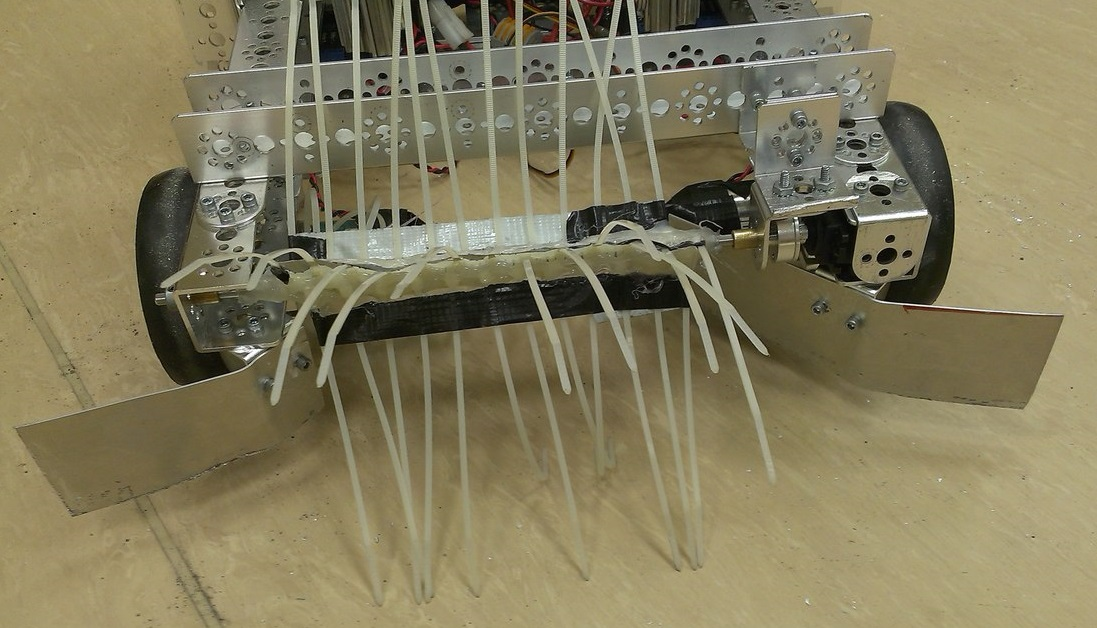
\includegraphics[scale=0.2]{days/24.10.14/images/01}}
      		\caption{Gripper with slopes}
      	\end{minipage}
      	\hfill
      	\begin{minipage}[h]{0.47\linewidth}
      		\center{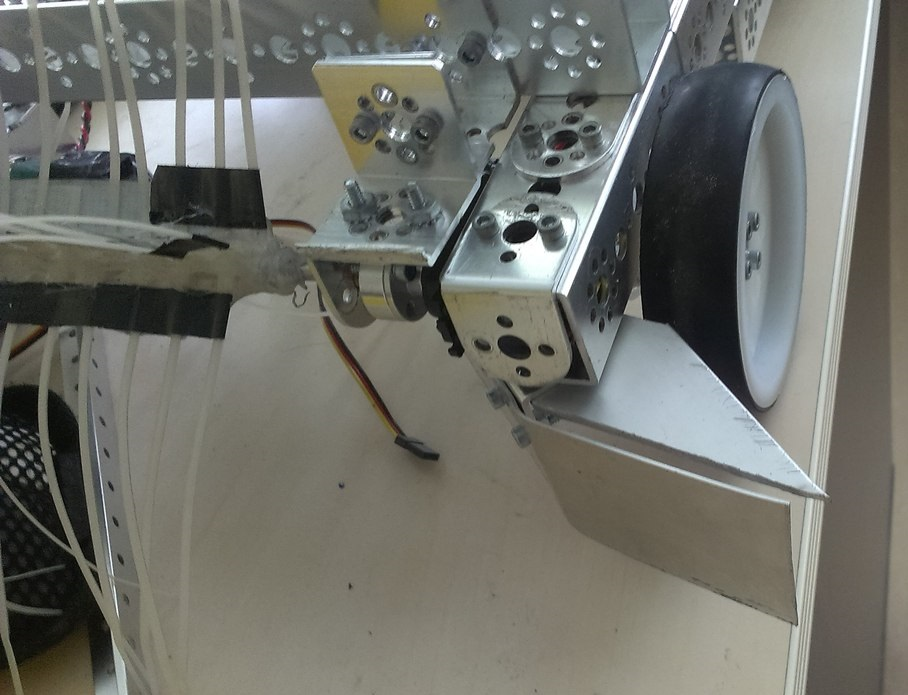
\includegraphics[scale=0.2]{days/24.10.14/images/02}}
      		\caption{Slopes with stops}
      	\end{minipage}
      \end{figure}
      
      \item Prepared the holes for installation of the remaining pair of crossbars at the lift.
      
    \end{enumerate}
    
	\item Results: 
	\begin{enumerate}
	  \item Problem with servo corrected.
	  
      \item Slopes for balls installed to robot.
      
    \end{enumerate}
    
	\item Tasks for the next congregations:
	\begin{enumerate}
	  \item To elaborate and create the mechanism of capture movable baskets.
	  
    \end{enumerate}     
\end{enumerate}
\fillpage
